\chapter{Plastic Flow in Silicon Nanowires}

\section{Discovery}

Within the ``wiring quantum dots'' project $Si$ nanowires where irradiated with $As^+$ and $In^+$ and/or $Ga^+$ so that in a subsequent annealing step $Si-GaAs$ or $Si-InGaAs$ hetero-structures could be formed. Markus Glaser, the Ph.D. student responsible for this part of the project, had developed a good habit of making SEM images of the same individual wires after each process step. We thus noticed, that the $Si$ nanowires shrank quite dramatically during the irradiation with $\approx 100\,keV$ $In^+$, $Ga^+$ and $As^+$ at room temperature. Two examples of this can be seen in figure \ref{deformSEM}. A look into literature revealed that this behavior has so far not been reported for irradiation of $Si$ at such low ion energies. A thorough investigation might be worthwhile. 
 
\begin{SCfigure}
	\centering
		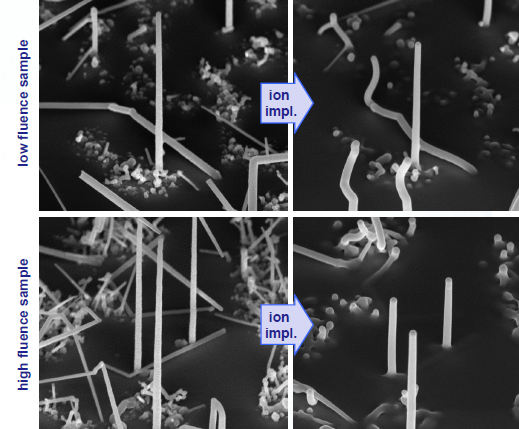
\includegraphics[width=.48\textwidth]{images/deformSEM.png}
	\caption{\textcolor{red}{placeholdergraph - get nicer image from Markus.} SEM images of VLS-grown $Si$-nanowires before and after the irradiation with X In and Y As at room temperature, while rotating the sample. The shrinking and widening of the wires is clearly visible. In the background wires which were not aligned perpendicular to the substrate are bent upward.} 
	\label{deformSEM}
\end{SCfigure}

Similar $Si$ nanowire arrays as the ones used for the sputtering experiment were thus systematically irradiated with $Ar^+$, making SEM images after each irradiated fluence to observe and quantify the deformation. $Ar$ was chosen for the irradiation to avoid any chemical effects and because it has a comparable mass to $Ga$ and $As$. Using the algorithm described in the sputter yield chapter, the profiles for the irradiated nanowires could be extracted. In figure \ref{deformationprofile} the black, red, green and blue lines indicate the height dependent diameter of a single wire before and after irradiation with $100\,keV\,\,Ar^+$ up to fluences of 1, 3 and $5 \times 10^{16}\,cm^{-2}$ respectively. In this graph, as well as in the inset black profiles, the reduction of the height by $\approx 500\,nm$ and an increase of the diameter, especially at the base, can be clearly seen. The deformation is only seen with irradiation at room-temperature where $Si$ amorphization threshold of $10^{14}\,ions/cm^2$ for $100\,keV\,\,Ar^+$ is very low \cite{pelaz_ion-beam-induced_2004}.

\begin{SCfigure}
	\centering
		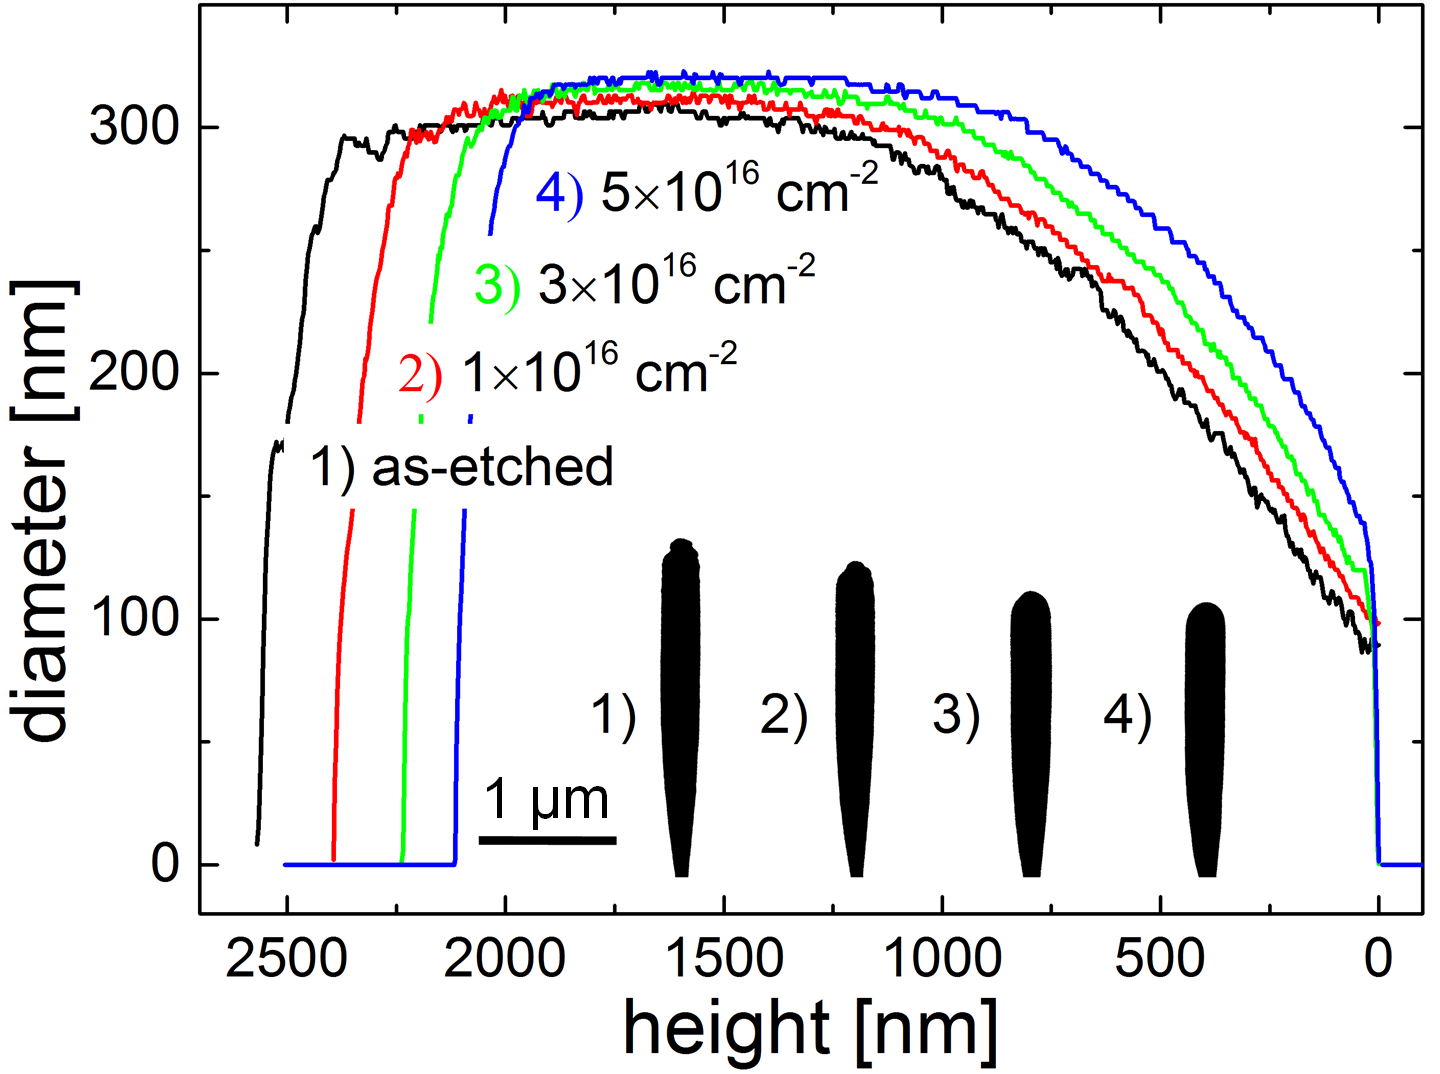
\includegraphics[width=.48\textwidth]{images/deformationprofile.jpg}
	\caption{Graphs of the diameter over height of a single $Si$ nanowire irradiated with increasing fluences of $100\,keV Ar^+$ ions. The black insets show the profiles of the nanowire after the respective fluences extracted from SEM images. In both illustrations the shrinking and widening of the wire is clearly visible.} 
	\label{deformationprofile}
\end{SCfigure}

\section{Quantification}

The deformation of the nanowires can be roughly quantified by fitting a linear trend to the fluence dependence of the height of the wires. This yields an average of $3\%$ shrinkage per $10^{16}\,ions/cm^2$. Due to outliers with larger deformation the values obtained for the 21 nanowires investigated have a large standard deviation of $\pm 3\%$ shrinking per $10^{16}\,ions/cm^2$. A more thorough investigation of the deformation is possible by also accounting for the height dependence of the diameter seen in figure \ref{deformationprofile}. On average a certain number of atoms are displaced by a certain distance along the height $z$ of the nanowire per ion. Considering only the movement along the height $z$, a mass-transport rate (MTR) can be calculated according to equation \ref{MRTequation}:

\begin{equation}  
\begin{split}
    MTR_{(1 \rightarrow 2)} & = [ {}^{1}N\cdot {}^{1}z_{c} -{}^{2}z_{c} \cdot {}^{2}N - ({}^{1}N - {}^{2}N) \cdot {}^{2}z_{c}]/N_{ion} \\
		& = {}^{1}N \cdot ({}^{1}z_{c} - {}^{2}z_{c})/N_{ion} 
	\label{MRTequation}
	\end{split}
\end{equation}

\begin{SCfigure}[50][h]
	\centering
		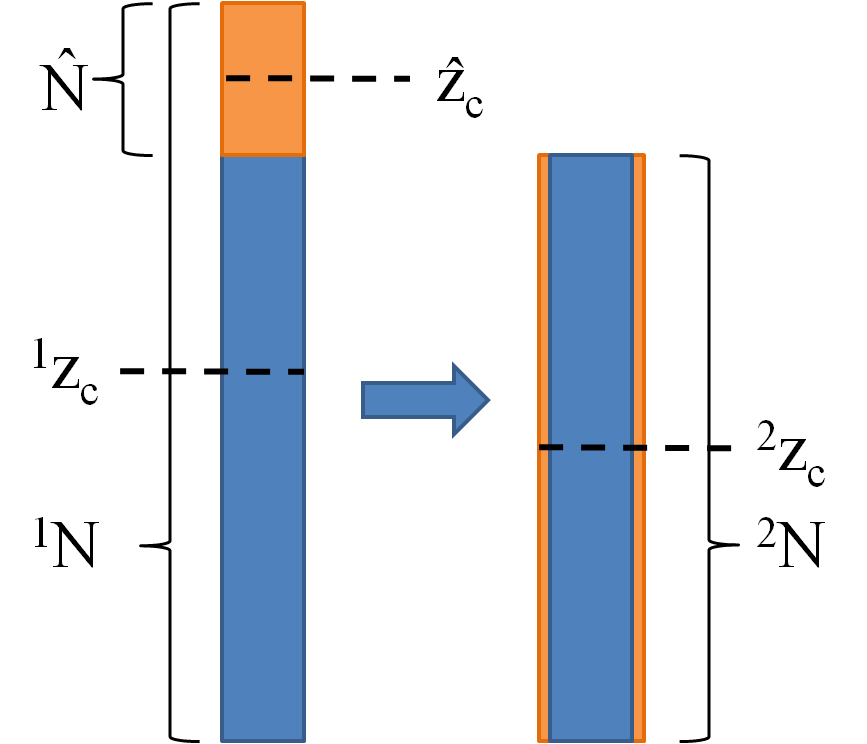
\includegraphics[width=.25\textwidth]{images/MTRillustration.png}
	\caption{Illustration of the mass-transport rate calculation. Displacing ${}^{1}N$ atoms from their average height ${}^{1}z_{c}$ to the average height ${}^{2}z_{c}$ requires the same mass-transport, as moving $\hat{N}$ from $\hat{z}_c$ to ${}^{2}z_{c}$, taking into account the sputtered atoms ${}^{1}N-{}^{2}N$.}
	\label{MTRillustration}
\end{SCfigure}

In equation \ref{MRTequation} and figure \ref{MTRillustration}, ${}^{1/2}z_{c}$ is the height of the center of mass of the nanowire with the top left index indicating before ($^1$) and after ($^2$) irradiation respectively. The number of atoms at height $z_i$ can be calculated from the local radius $r_i$. Summing up the height weighted by the number of atoms at that height $z_{c} \cdot N = \sum_i{\pi r_i^2 h \cdot \rho \cdot z_i}$ and dividing this by the total number of atoms $N = \sum_i{\pi r_i^2 h \cdot \rho}$ in the nanowire gives us $z_{c}$. The sums are over all slices $i$ of height $h = 1\,pixel = 2.7\,nm$ (typically) each. The number of ions that hit the nanowire in the irradiation of fluence $\Phi_{12}$ between making SEM images $1$ and $2$ is $N_{ion} = \sum_i{({}^{1}r_i+{}^{2}r_i)}$ $\cdot sin(45^\circ) \cdot h \cdot \Phi_{12}$. The last term in equation \ref{MRTequation} accounts for the influence of sputtered atoms. Just as in the chapter on sputtering, the sputter yield could be calculated by $({}^{1}N - {}^{2}N)/N_{ion}$. Figure \ref{MTRillustration} illustrates two interpretations of the MTR calculation. As only the displacement along $z$ is considered, the direct interpretation of equation \ref{MRTequation} of moving ${}^{1}N$ atoms from their center of gravity ${}^{1}z_{c}$ to a new center of gravity ${}^{2}z_{c}$ is equivalent to moving the atoms which are `missing' at the top of the wire after the irradiation ($\hat{N}$, orange volume in figure \ref{MTRillustration}) from their center of gravity $\hat{z}$ to ${}^{2}z_{c}$, and subtracting the sputtered atoms. This evaluation yields an average mass-transport rate of $1.2\cdot10^4 \,atoms \cdot  nm / ion$ with a standard deviation of $7\cdot 10^3\,atoms \cdot nm / ion$. Again the large standard deviation is due to outliers with larger deformation.

\section{Knock-on transport of mass}

A possible explanation for this behavior can be sought in the linear cascade theory which is applicable for the cascades of $100\,keV\,\,Ar^+$ in $Si$. In a collision cascade following an energetic ion impinging a solid, atoms will be preferentially `knocked-on' along the propagation direction of the impinging ion. This causes an inhomogeneous distribution of interstitials and vacancies and effectively mass is transported `downstream' along the ion beam. In an amorphous material it is not clear what constitutes an `interstitial' or a `vacancy', but a local excess of vacancies can be understood as a locally decreased density, while an interstitial excess corresponds to an increased density. A local density gradient is not stable, since the density of amorphous $Si$ before and after irradiation is not significantly different \cite{pelaz_ion-beam-induced_2004}. Therefore, the density gradient introduces stress in the material which can relax by plastic deformation, possibly enabled by a decreased viscosity due to further ion irradiation \cite{snoeks_stress_1997,hu_burrowing_2002,mayr_mechanisms_2003,mayr_effect_2003}. 

As was shown in the example of sputtering, BCA simulation software can accurately reproduce linear collision cascades. Therefore, comparing the experiments with a simulation with \emph{iradina} can evaluate whether the deformation observed in the experiment can be accounted for by knock-on mass transport. Figure \ref{deformationBCA}a shows the simulation volume implemented in \emph{iradina} with $2\times2\times2\,nm^3$ voxels as a $600\,nm$ long $Si$ cylinder with a diameter of $200\,nm$. The $100\,keV\,\,Ar^+$ ions impinge at an angle of $45^\circ$ to the $z$-axis. They strike the cylinder distributed uniformly along the $y$-direction at height $z=0$. Figure \ref{deformationBCA}d shows the resulting distribution of interstitials on the cross-sectional slice through the middle of the nanowire along the $xz$ plane. This can be seen as an approximation for the distribution of the nuclear energy loss and shows the mean extent of the collision cascade. Figure \ref{deformationBCA}e shows the same cross-section after subtracting the number of vacancies produced per ion from the number of interstitials. The excess of vacancies along the impinging plane (blue cone in the cross section) enveloped by two red planes of excess interstitials shows that there is a high probability for the ions to hit a target atom with a large impact parameter. This changes the ions path only little and displaces the target atom in an direction perpendicular to the ion beam. Superimposing many collisions along the $y$ direction leads to the formation of one one vacancy rich and two interstitial rich planes. The $xy$-plane in \ref{deformationBCA}b shows the sum over the height $z$ of the difference between interstitials and vacancies plotted to the same color scale. The illustration is dominated by vacancies at the surface of the cylinder which are left behind by sputtered atoms. 

The height distribution (summing over the radial $xy$ plane) of the interstitials, vacancies and leaving atoms is shown in \ref{deformationBCA}c. As expected, the majority of sputtered atoms originate near the impact height. The lines showing the interstitials and vacancies overlap in this illustration. The vacancies subtracted from the sum of interstitials and leaving atoms is plotted along the height in \ref{deformationBCA}f. As a displaced atom, leaving behind a vacancy, is either sputtered or becomes an interstitial, the sum over all heights of of this graph is zero. The strong oscillation around $z=0$ in \ref{deformationBCA}f is caused by the previously discussed displacement of target atoms at an angle almost perpendicular to the ion beam for large impact parameters. This oscillation is very sensitive to the voxel-size as in effect the voxel size defines a recombination length and interstitial and vacancy rich regions are mixed in larger voxels. On the other hand, the excess of vacancies near the impact point ($\le 70\,nm$) and of interstitials further down along the ion's path ($\approx 100\,nm$) is not sensitive to the voxel size. It can be used to quantify the knock-on mass transport by multiplying the plotted values by their height and integrating over all heights. The influence of the short range oscillation immediately around the impact point disappears as here $z \approx 0$ is small. The value obtained from this calculation is $78\pm1\,atoms \cdot nm /ion$. Clearly this value is to low to account for the large deformation observed in the experiment where a mass-transport rate of $\ge 1\times 10^{4}\,atoms \cdot nm /ion$ was assessed.

\clearpage
\begin{figure}[thbp]
	\centering
		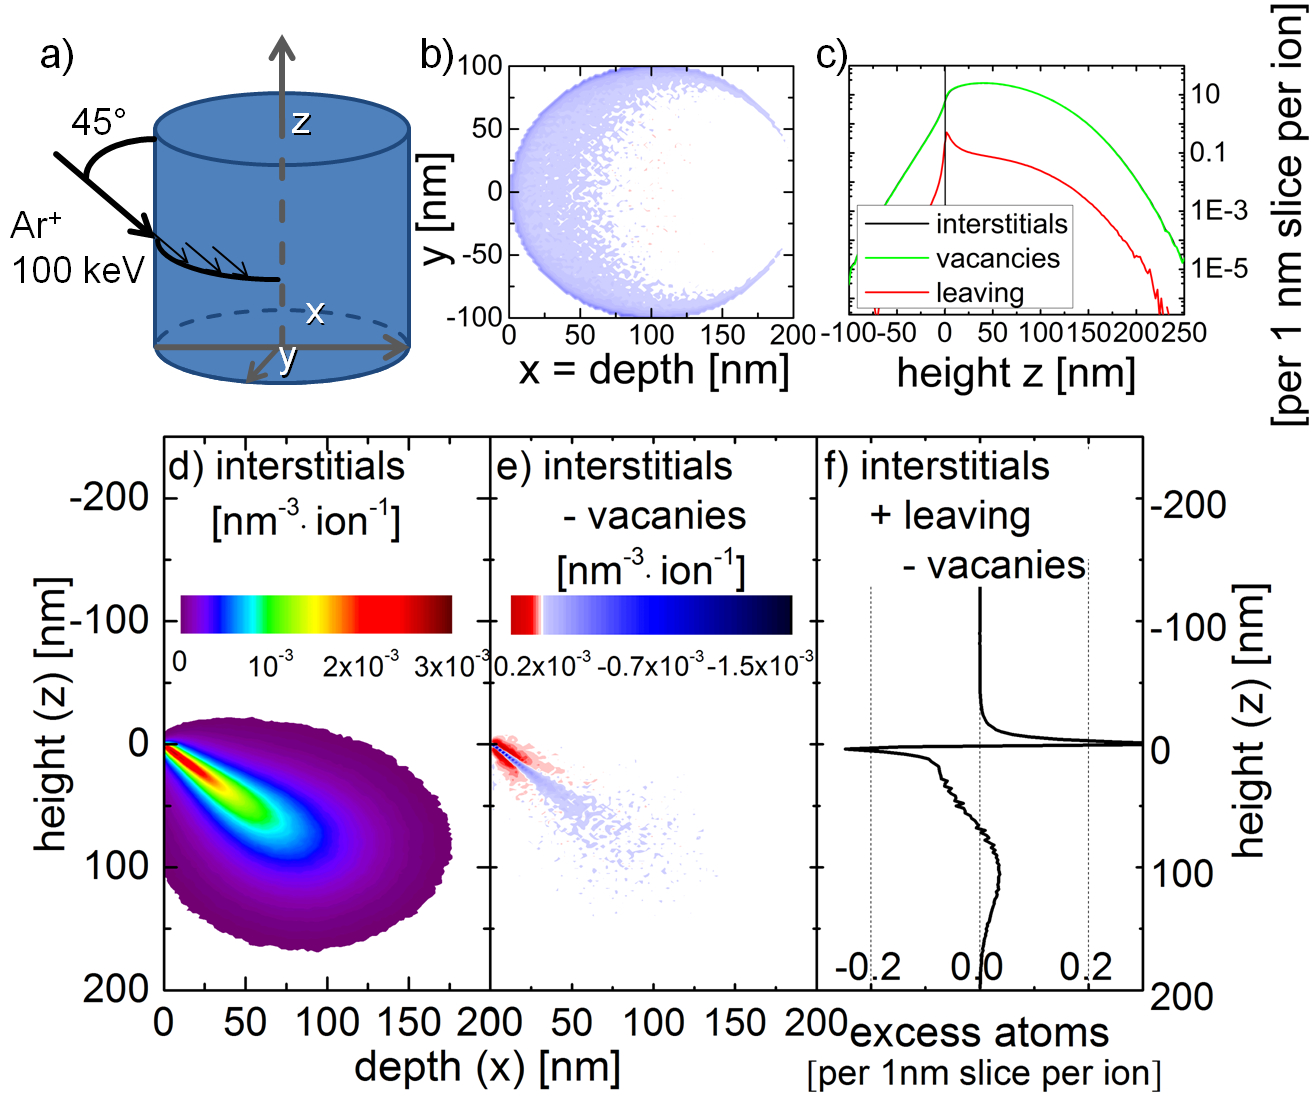
\includegraphics[width=8cm]{images/deformationBCA.jpg}
		\caption{a) Illustration of the simulated irradiation geometry. All $Ar^+$ ions of $100\,keV$ energy hit the nanowire volume at the same height and at an angle of $45^\circ$ with respect to the wire axis $z$. The created interstitials in the radial cross-section through the middle of the simulated nanowire is shown in d). This distribution is effectively an illustration of the nuclear energy loss. In e) the vacancies are subtracted from the interstitials for the same cross-section. Summing this difference over all heights gives the radial distribution shown in b). The clear dominance of vacancies near the surface is caused by sputtering. The axial profile of the interstitials, vacancies and leaving (sputtered) atoms plotted in c) over the height relative to the impact plane shows that most atoms are sputtered at the impact height. Note that the plots of vacancies and interstitials overlap. The vacancies subtracted from the sum of interstitials and sputtered atoms plotted over the height in f) shows mass transport along the ion's path. Apart from the strong oscillation at the impact height, there is a deficiency of atoms close to the impact height ($\le 70\,nm$) and an excess centered around $100\,nm$ down from the impact height.} 
	\label{deformationBCA}	
\end{figure}

For all simulations a reasonable value for crystalline $Si$, $15\,eV$ \cite{corbett_production_1965}, was used for the displacement energy which governs the creation of interstitials and vacancies in the simulation, as discussed in chapter \ref{sec:simion}. However, in amorphous materials it is questionable what this value is supposed to mean, as point defects are not well defined. Therefore, simulations where repeated with the displacement energy set to $0\,eV$. As expected, the number of `vacancies' and `interstitials' now produced by the simulation increased dramatically. However, the long range difference between `vacancies' and `interstitials' seen in figure \ref{deformationBCA}f is unchanged. This is an indication that the knock-on mass transport is dominated by the rare events where target atoms are hit directly by the impinging ions. In these cases, a large amount of energy is transferred to the displaced atom leading to a long trajectory within the material. The atoms displaced with lower energies are much more numerous, but travel much shorter distances and in a randomly orientated direction. This is because most of the low energy displaced atoms are generated at the end of a branch of the collision cascade, the orientation of the branch having previously been randomized by higher energy collisions. And/or they originate from collisions with a high impact factor, which lead to a large angle between the incoming particle's and the displaced particle's momentum, as seen in the separation of interstitials and vacancies near the impact point in figure \ref{deformationBCA}e.

\section{Irradiation at large angles of incidence}

If knock-on mass-transport is not the main contribution to the deformation, the question arises whether the direction of the deformation is related to the ion beam. Will an irradiation from `below the substrate' towards an unconstrained end of the nanowire would also shrink the wire, or stretch it out? Nanowires attached to a substrate are obviously not suited to testing this, so a method to irradiate nanowires while rotating them at angles greater than $90^\circ$ to the ion beam was devised. This was achieved by attaching a $Si$ nanowire grown epitaxially on a $Si$ wafer to an $Au$ microwire which can suspend the nanowire at arbitrary angles in the irradiation chamber. The process is shown in figure \ref{reverseFIB}. The $Pt$ deposition was used to glue the nanowire to the micro-manipulator in the FIB and cut the nanowire from the substrate with the $Ga$-FIB. Using the $Pt$-deposition and $Ga$-FIB again, the nanowire is subsequently attached to the tip of a sharpened $Au$-microwire which was previously glued to a piece of wafer for handling and also placed in the FIB chamber. VLS-grown nanowires were used for this experiment as they were readily available in longer lengths ($>10\mu m$) than the etched nanowires.

\begin{figure}[thbp]
	\centering
		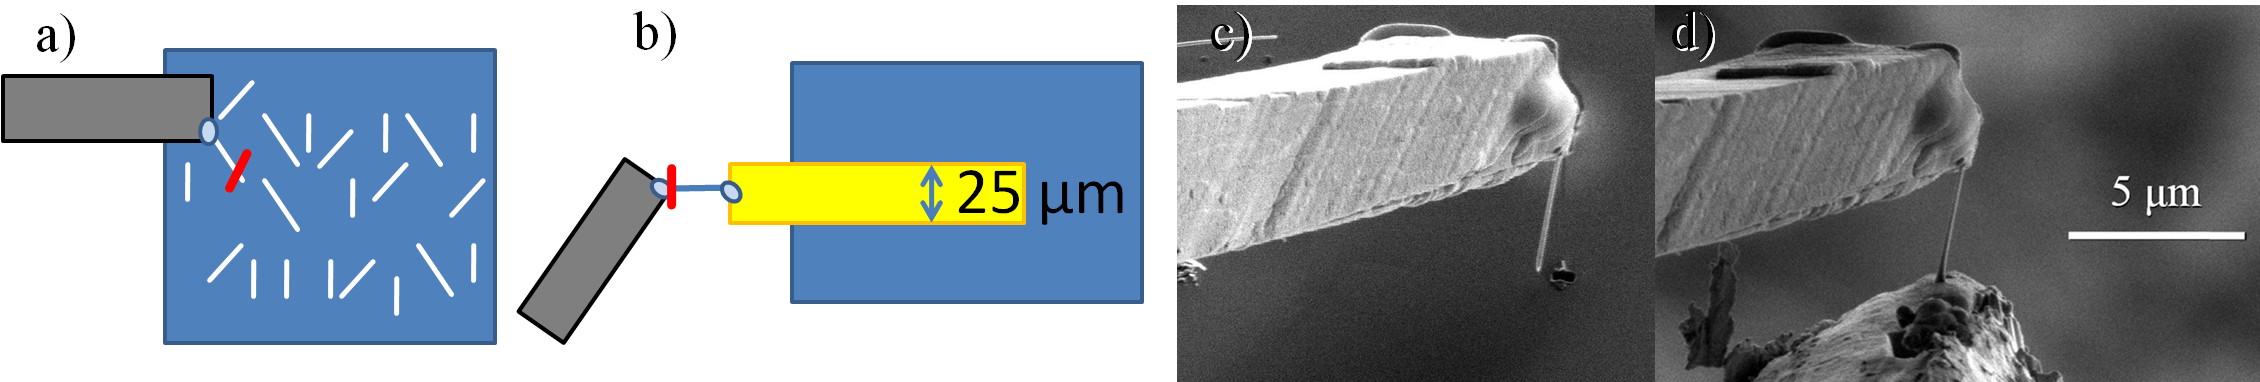
\includegraphics[width=0.99\textwidth]{images/reverseFIB.jpg}
	\caption{Illustration of the nanowire-on-microwire fabrication in a FIB system. The schematic a) and SEM image c) show the wire first glued to the micro-manipulator in the FIB by $Pt$-deposition (light blue ellipse), then cut from the substrate with the $Ga$-FIB (red line). Images b) and d) Illustrate the subsequent gluing to an $Au$ microwire with $Pt$-deposition and the final cut with the $Ga$-FIB to release the nanowire from the micro-manipulator.}
	\label{reverseFIB}
\end{figure}

The nanowire-on-microwire samples consisted of typically $3-5$ nanowires, each attached to an $Au$-microwire and arranged in the irradiation chamber on a rotatable stage at an angle of $135^\circ$ to the ion beam, as shown in figure \ref{reverseangle}a. The alignment of the nanowires to their microwire support was found to be crucial, as any shadowing of a nanowire from the ion beam an one side would lead to extreme bending of the wire. Only a single wire was found straight enough to evaluate quantitatively for more than on irradiation step. The SEM images of this wire are shown in figure \ref{reverseangle}b-f view from a perspective perpendicular to the axis of rotation and rotated by the indicated angle around this axis. The left SEM images show the uniradiated nanowire, while the center and right images were made after the irradiation of $1\times10^{16}\,cm^{-2}$ and $3\times10^{16}\,cm^{-2}$ $100\,keV\,\,Ar^+$, respectively. The uniradiated wire is straight and $3.9\,\mu m$ long. The irradiated wire shows some bending, so the length had to be determined from a perspective were the curvature of the wire is in plane with the image. A fifth order polynomial was fitted to the bent shape and the length of the wire was thus determined to be $3.5\,\mu m$ after $1\times10^{16}\,cm^{-2}$ (\ref{reverseangle}b) and $3.2\,\mu m$ after $3\times10^{16}\,cm^{-2}$ (\ref{reverseangle}f). The nanowire thus shrank with a similar deformation rate to the previously reported $3\%$ strain per $10^{16}\,ions/cm^2$, even though the irradiation was directed towards its free end.

\begin{figure}[thbp]
	\centering
		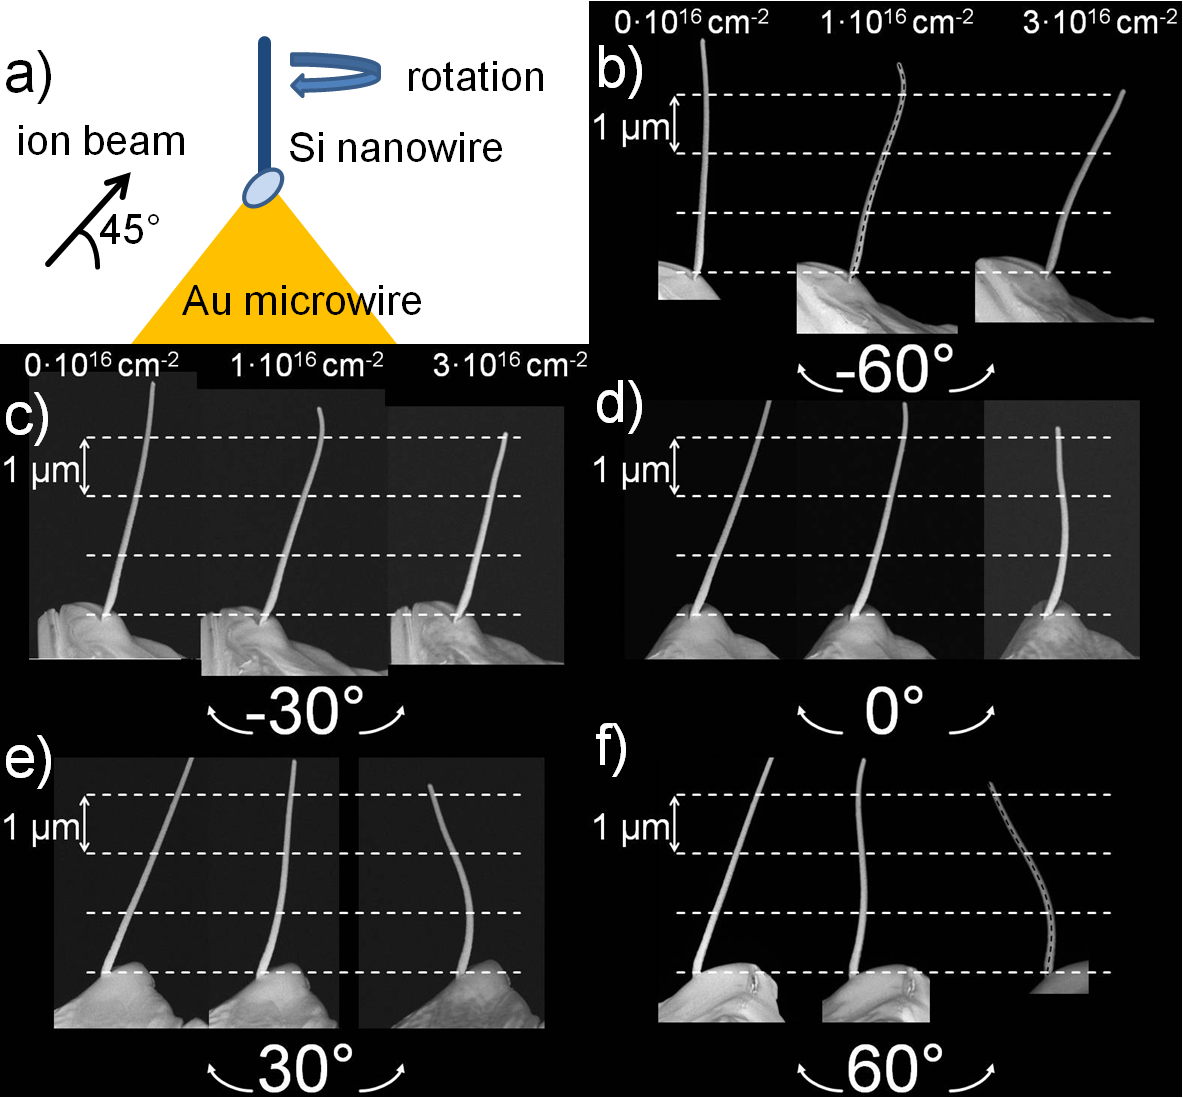
\includegraphics[width=8cm]{images/reverseangle.jpg}
	\caption{ a) Illustration of the nanowire-on-microwire irradiation setup. b) - f) SEM images of the same nanowire as-mounted (left SEM images), after irradiation with $1\times10^{16}\,cm^{-2}$  (center images), and $3\times10^{16}\,cm^{-2}$ (right images) $\,100\,keV Ar^+$ ions. The SEM images where taken with the nanowire rotated by the indicated angle from a perspective perpendicular to the angle of rotation. The length of the nanowire after irradiation is determined in b) and f) along the dashed lines.}
	\label{reverseangle}
\end{figure}

This experiment shows with certainty that the knock-on mass-transport is not the main contributor to the observed deformation, as it would have to be directed along the ion beam. The discussion of a possible model for the deformation will be easier by addressing similar effects and the way that simulation tools were used to understand them. The BCA MC simulation tools available inherently neglect all collective movement of atoms within the target. As has been shown in the previous two chapters, this may be sufficient for the prediction of sputtering and the ion distribution in nanostructures. A field of study which has already faced the limitation of neglecting the local temperature in ion irradiation is the irradiation with swift, heavy ions. At energies well beyond $MeV$ the assumption that the dominating effects will be described by binary collisions between the ion and target atoms is false. At these high energies and ion masses a significant amount of energy will be transferred form the ion to the electronic system of the target. Through the relaxation mechanisms of the electronic system a part of this energy will be converted to heat in the lattice. Under certain conditions this will form ``ion-tracks'' in the target. One approach to understanding the formation and behavior of ion-tracks is to simulate the longitudinal distribution of the deposited ion energy in the target with BCA tools (typically SRIM) and to evaluate the local temperature in a second step by following the deposited energy according to thermodynamic considerations. A good review of such ``thermal spikes'' can be found in \cite{wesch_effect_2004}. 

Such a thermal spike approach was successful at understanding the plastic deformation by swift heavy ion irradiation according to Trinkaus and Ryazanov \cite{trinkaus_viscoelastic_1995} and in the understanding of material properties governing the direction of the deformation \cite{hedler_amorphous_2004,hedler_boundary_2005}. When nanoparticles are deformed \cite{snoeks_colloidal_2000,snoeks_colloidal_2001,van_dillen_anisotropic_2001,dillen_energy-dependent_2001,dillen_ion_2003,dillen_ion_2004} an adapted version of the model by Trinkaus can be applied and the effect dubbed ``ion hammering'' \cite{klaumunzer_ion_2004}. In short, according to this model the local temperature leads to a transient `liquid' phase in the cylindrical volume of material around the ion's path. Within the cylindrical geometry, the deformation by thermal expansion is anisotropic and because stresses can relax in the low viscosity volume, this is a plastic deformation. This is not observed in materials which remain crystalline during the irradiation, as the long range order of the crystal lattice is reinforced upon the recrystallization during cooling. The problem with directly applying this model to the situation at hand is that the total energy density in the collision cascade of $100\,keV\,Ar^+$ in $Si$ is a low $\frac{dE}{dx} = 36\,\frac{eV}{nm}$, of which the electronic energy loss is roughly half. Also, the lowest ion energy for which plastic deformation of silica nanoparticles is reported is $300\,keV Xe^+$ \cite{dillen_ion_2003}. Here the energy loss is merely $\frac{dE}{dx} = 120\,\frac{eV}{nm}$ with $20\,\%$ lost to the electronic system. The threshold for ion tracks, however, is given at $\frac{dE}{dx} \geq 1\,\frac{keV}{nm}$ by Trinkaus et al. \cite{trinkaus_viscoelastic_1995}!

The alternative to thermodynamic considerations after a MC BCA simulation are full MD simulations, where the trajectory and interaction of every atom or ion in the simulation volume is followed. This naturally includes all thermal effects, but is limited by computing power to a low number of atoms and thus a severely limited volume of material. Additionally the accuracy of results depends greatly on finding the interaction potential for all combinations of ions and atoms involved. Here again, as for sputtering, this is true especially for low energy interactions, where these potentials are not available but a topic of research in themselves \cite{primetzhofer_inelastic_2012,primetzhofer_local_2013}. Investigations of the self-irradiation of $10\,keV\,Si$ and various metals \cite{nordlund_defect_1998} revealed the formation of nanoscale `liquid' pockets. The term ``liquid'' must be used with care as it refers to a thermodynamical state of matter while the simulation timescale does not allow the assumption of thermodynamic equilibrium. Nevertheless, a sufficiently large number of atoms gain much kinetic energy (say `are hot') to make the assumption of reduced viscosity and other effects safe. The interesting point of this example is that the energy in the collision cascade was quite low, so that the trajectory of the initiating particle could also have been accurately simulated according to the BCA. A more recent MD investigation by Baumer et al. gets even a step closer to the presented experimental results, in that it predicts plastic deformation in metallic glasses irradiated with high energy neutrons \cite{baumer_prediction_2014}. The collision cascades are initiated in $a$-$Cu_{50}Nb_{50}$ by assuming primary knock-on atoms of $475\,keV Nb$. This atomistic study explicitly shows that plastic deformation due to thermal expansion and stress relaxation can be anisotropic also in collision cascades which do not have the high energy density and symmetry required by the Trinkaus model \cite{trinkaus_viscoelastic_1995}. Somewhat contrary results were obtained by Mayr et al. \cite{mayr_mechanisms_2003} where $10\,eV$ to $100\,keV$ recoils of $Cu$ and $Ti$ in $a$-$CuTi$ were simulated. That study comes to the conclusion that the viscous flow is dominated by ion induced point defects. It does not propose that knock-on atoms are initiate the deformation, but rather, that thermal effects do not provide the main contribution to the reduced viscosity observed during ion irradiation.


\begin{figure}[thbp]
	\centering
		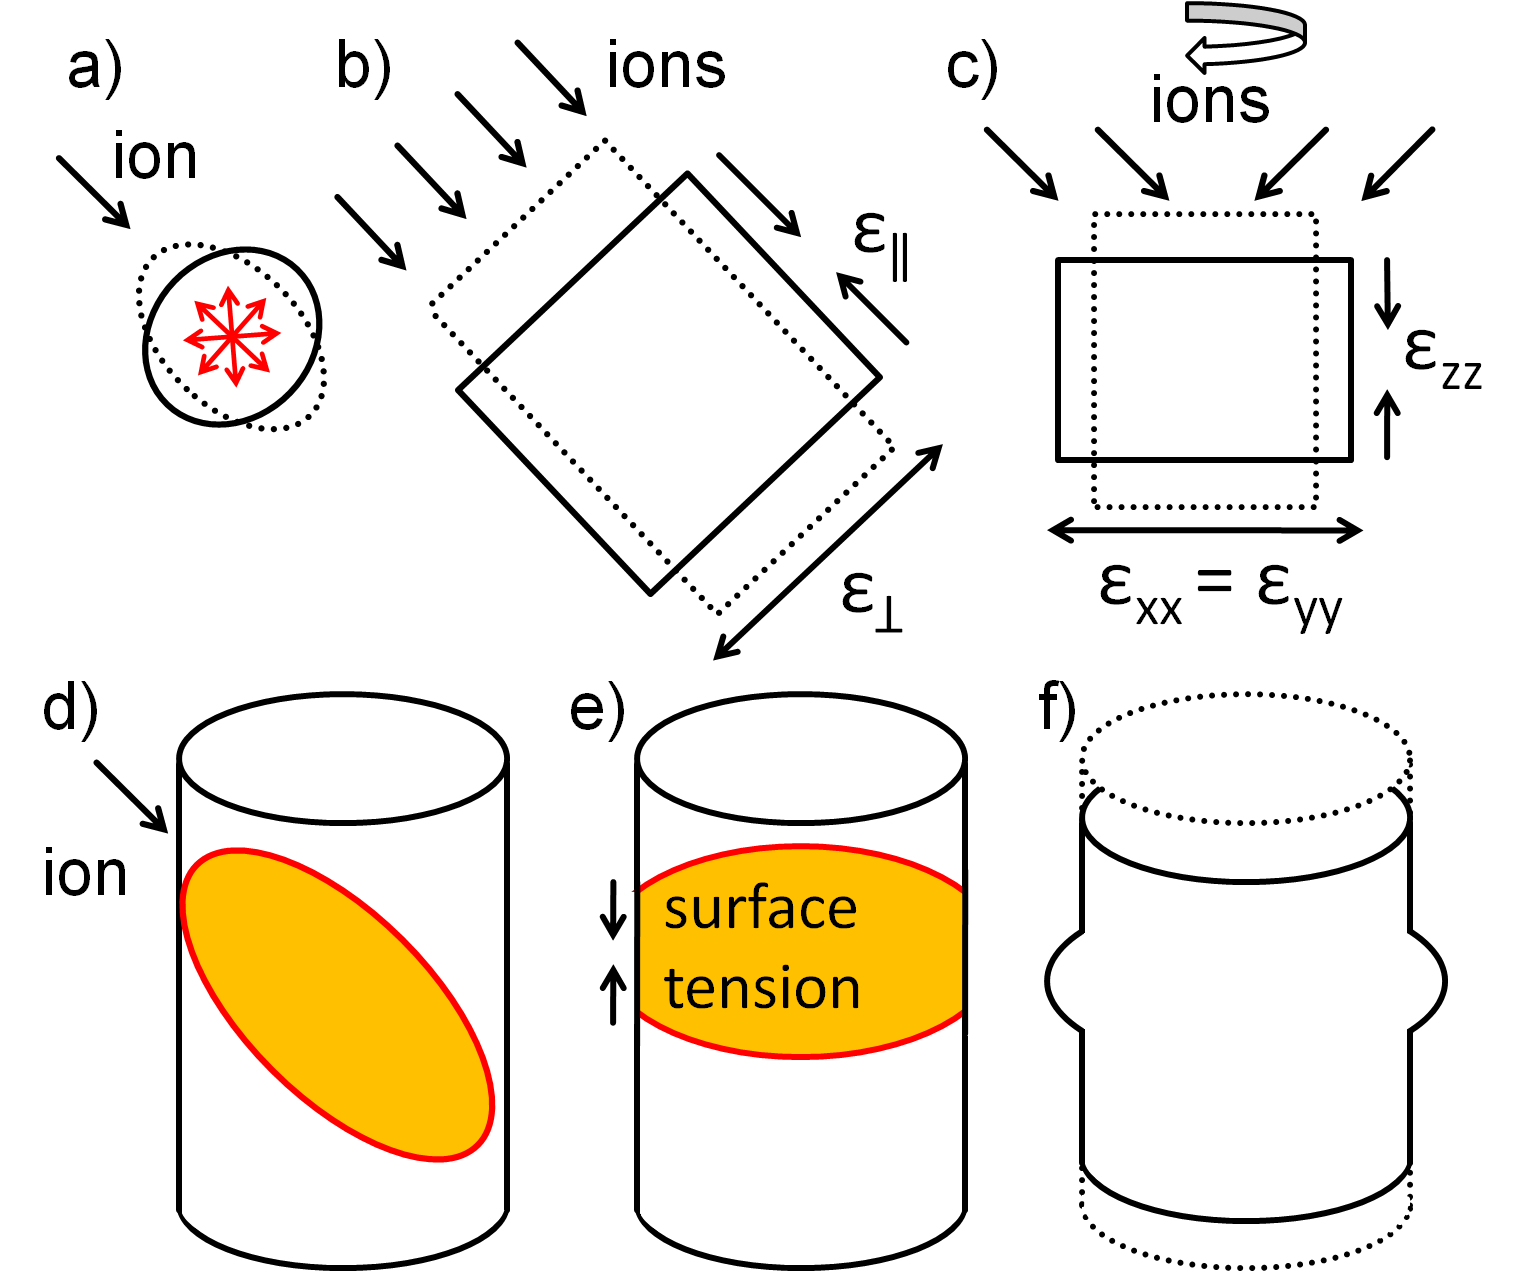
\includegraphics[width=8cm]{images/deformationmodel.jpg}
	\caption{a) - c) Illustration of a deformation model analogous to ion hammering. a) The collision cascade from a single impinging ion heats an approximately ellipsoidal volume of the target material. The internal pressure will lead to an expansion towards a more spherical shape which is retained upon cooling. b) The net effect of many ions is thus a contraction parallel to and an expansion perpendicular to the ion beam. For no change in density $\epsilon_\parallel = -2\epsilon_\perp$ has to hold. c) Under rotational symmetry this deformation translates to a contraction in the rotational axis $z$ and an expansion in the perpendicular $x-y$ plane with $\epsilon_{zz} = -2\epsilon_{xx} = -\epsilon_\perp$. In d) - f) the alternative, surface tension driven deformation is illustrated. The collision-heated volume of target material shown in d). A significant slice of the wire shown in e) thus has a reduced viscosity. The surface energy is reduced by an increase in the local diameter of the wire, leading to a shortened and thickened wire segment shown in f).} 
	\label{deformationmodel}
\end{figure}

\section{The deformation mechanism}

The effect of anisotropic deformation within the collision cascade induced by the irradiation of nanowires is shown in figure \ref{deformationmodel}a - c. An approximately ellipsoidal volume of the target material is heated by the collision cascade. It expands, becoming more spherical and the anisotropic deformation is retained after cooling. The superimposition of many collision cascades with a similar effect leads to a net contraction along the ion beam $\epsilon_{\parallel} < 0$ and an expansion perpendicular to it $\epsilon_{\perp} > 0$ as shown in \ref{deformationmodel}b. To maintain constant density $-2\cdot\epsilon_{\perp} =  \epsilon_{\parallel}$. The rotational average of this deformation around the $z$-axis, as illustrated in \ref{deformationmodel}c, works out to be a contraction along the $z$-axis $\epsilon_{zz} = \frac{1}{2} \epsilon_{\parallel}$ and a corresponding expansion in the $xy$-plane for an angle of $\pm\, 45^\circ$ between the ion beam and the $z$-axis. The $z$-axis represents the nanowire axis, while the $xy$-plane is parallel to the nanowire diameter. Thus the deformation rate of $\frac{d\epsilon_{zz}}{d\Phi} = 3\%$ strain per $10^{16}\,ions/cm^2$ extracted from a linear fit to the reduction of the nanowire height can be transformed into a strain rate parallel to the ion beam of $\frac{d\epsilon_{\parallel}}{d\Phi} = 6\%$ strain per $10^{16}\,ions/cm^2$. This is much less than the values reported for the studies at higher energies reported in literature. In ref. \cite{dillen_ion_2003} $10^{-16}\,cm^2/ion$ were reported for $300\,keV\,Xe$ in silica nanoparticles and ref. \cite{baumer_prediction_2014} even arrives at $10^{-15}\,cm^2/ion$ with MD calculations in bulk. There are unfortunately no studies published on straining bulk silicon at these low ion energies. The bending of thinned $Si$-wafers similar to \cite{volkert_stress_1991,massl_stress_2008} would be measurable with the a straining rate of $6\%$ strain per $10^{16}\,ions/cm^2$ in a layer of $\approx 300\,nm$.

The quantitative discrepancy between the deformation observed in the experiments presented here and published studies may be attributed to the lower ion energy and one may gain confidence in this model due to the qualitative similarity to the MD simulations by Baumer et al. \cite{baumer_prediction_2014} also showing deformation anisotropy at relatively low ion energies. However, a further, major concern is the fact that in the presented experiments the collision cascade is not in bulk, but in a nanostructure were there is not much material around and it is not distributed around the cascade isotropically. If the ellipsoidal volume intersects the nanowire surface, the pressure from the thermal expansion will vent outward removing the force needed to drive the deformation. An more favorable model illustrates that the strong influence of the surface expected in nanowires can also lead to the observed plastic deformation. In figure \ref{deformationmodel}d the relation between the nanowire and collision cascade is shown. As there is not much material around, the temperature in a sizable slice of the nanowire will remain elevated for some time \cite{borschel_ion-solid_2012,greaves_enhanced_2013,anders_sputtering_2015,johannes_ion_2015}. In addition the ion irradiation will further reduce the viscosity \cite{snoeks_stress_1997,hu_burrowing_2002,mayr_mechanisms_2003}, allowing the surface tension to deform the nanowire by increasing the radius locally. The local increase in diameter reduces the total surface area and thus the surface energy. The wire subsequently becomes shorter and wider as shown in figure \ref{deformationmodel}f. 

Apart from the bulk deformation experiment already suggested, a further experiment which could distinguish which of the two models applies is the irradiation of the nanowires at $90^\circ$ between the nanowire axis and the ion beam. In this case if the first model similar to ion hammering applies the irradiation should produce slowly elongating wires with a reduced radius, as the positive $\epsilon_{\perp}$ is now parallel to the nanowire axis. On the other hand, if the surface tension driven model is applicable the nanowires will shrink regardless of the irradiation angle. Naturally, a similar nanowire-on-microwire setup to the one for irradiation at $135^\circ$ could be used to irradiate at $90^\circ$. It turns out however, that the irradiation at $90^\circ$ is extremely prone to bending the nanowires. Due to the bending, the angle between the nanowire and the ion beam varied during a rotation cycle so that a conclusive discrimination between the models can unfortunately not be made. The bending can be attributed to the $Pt$ deposited to glue the $Si$ nanowire onto the $Au$ microwire in the FIB. This deposition is concentrated at the base and on one side of the nanowire and thus suppresses the rotational symmetry of the deformation, leading to bending. In the irradiation at $135^\circ$ the base of the wire, where it is glued to the microwire, is shadowed from the ion beam by the microwire so that the nanowires are less likely to bend. 
